%!TEX TS-program = xelatex
% !TeX program = xelatex
%!TEX encoding = UTF-8 Unicode
%----------------------------------------------------------------------------------------
%   Доорх хэсгийг өөрчлөх шаардлагагүй
%----------------------------------------------------------------------------------------
\documentclass[12pt,A4]{report}

\usepackage{fontspec,xltxtra,xunicode}
\setmainfont[Ligatures=TeX]{Times New Roman}
\setsansfont{Arial}

% \usepackage[utf8x]{inputenc}
% \usepackage[mongolian]{babel}
%\usepackage{natbib}
\usepackage{geometry}
%\usepackage{fancyheadings} fancyheadings is obsolete: replaced by fancyhdr. JL
\usepackage{fancyhdr}
\usepackage{float}
\usepackage{afterpage}
\usepackage{graphicx}
\usepackage{amsmath,amssymb,amsbsy}
\usepackage{dcolumn,array}
\usepackage{tocloft}
\usepackage{dics}
\usepackage{nomencl}
\usepackage{upgreek}
\newcommand{\argmin}{\arg\!\min}
\usepackage{mathtools}
\usepackage[hidelinks]{hyperref}

\usepackage{algorithm}
\usepackage{algpseudocode}

\usepackage{listings}
\DeclarePairedDelimiter\abs{\lvert}{\rvert}%
\makeatletter
\usepackage{caption}
\captionsetup[table]{belowskip=0.5pt}
\usepackage{subfiles}

\usepackage{listings}

\usepackage{color}
\definecolor{lightgray}{rgb}{.9,.9,.9}
\definecolor{darkgray}{rgb}{.4,.4,.4}
\definecolor{purple}{rgb}{0.65, 0.12, 0.82}

\lstdefinelanguage{JavaScript}{
  keywords={abstract, any, as, boolean, break, case, catch, class, console, 
    const, continue, debugger, declare, default, delete, do, else, enum, export, 
    extends, false, finally, for, from, function, get, if, implements, import, in, 
    infer, instanceof, interface, keyof, let, module, namespace, never, new, null, 
    number, object, package, private, protected, public, readonly, require, return, 
    set, static, string, super, switch, symbol, this, throw, true, try, type, typeof, 
    undefined, unique, unknown, var, void, while, with, yield,async},
  keywordstyle=\color{blue}\bfseries,
  ndkeywords={class, export, boolean, throw, implements, import, this},
  ndkeywordstyle=\color{darkgray}\bfseries,
  identifierstyle=\color{black},
  sensitive=false,
  comment=[l]{//},
  morecomment=[s]{/*}{*/},
  commentstyle=\color{purple}\ttfamily,
  stringstyle=\color{red}\ttfamily,
  morestring=[b]',
  morestring=[b]"
}

\lstset{
   language=JavaScript,
   backgroundcolor=\color{lightgray},
   extendedchars=true,
   basicstyle=\footnotesize\ttfamily,
   showstringspaces=false,
   showspaces=false,
   numbers=left,
   numberstyle=\footnotesize,
   numbersep=9pt,
   tabsize=2,
   breaklines=true,
   showtabs=false,
   captionpos=b
}
\renewcommand{\lstlistingname}{Код}
\renewcommand{\lstlistlistingname}{\lstlistingname ын жагсаалт}

\usepackage{color}
\definecolor{codegreen}{rgb}{0,0.6,0}
\definecolor{codegray}{rgb}{0.5,0.5,0.5}
\definecolor{codepurple}{rgb}{0.58,0,0.82}
\definecolor{backcolour}{rgb}{0.99,0.99,0.99}
 
\lstdefinestyle{mystyle}{
    basicstyle=\ttfamily\small,
    backgroundcolor=\color{backcolour},   
    commentstyle=\color{codegreen},
    keywordstyle=\color{magenta},
    numberstyle=\tiny\color{codegray},
    stringstyle=\color{codepurple},
    %basicstyle=\footnotesize,
    breakatwhitespace=false,         
    breaklines=true,                 
    captionpos=b,                    
    keepspaces=false,                 
    numbers=left,                    
    numbersep=10pt,                  
    showspaces=false,                
    showstringspaces=true,
    showtabs=false,                  
    tabsize=2
}
 
\lstset{style=mystyle, label=DescriptiveLabel} 

\let\oldabs\abs
\def\abs{\@ifstar{\oldabs}{\oldabs*}}
\makenomenclature
\begin{document}


%----------------------------------------------------------------------------------------
%   Өөрийн мэдээллээ оруулах хэсэг
%----------------------------------------------------------------------------------------

% Дипломийн ажлын сэдэв
\title{Веб програм хөгжүүлэлт}
% Дипломын ажлын англи нэр
\titleEng{Full-stack web development}
% Өөрийн овог нэрийг бүтнээр нь бичнэ
\author{Даянгийн Балжинням}
% Өөрийн овгийн эхний үсэг нэрээ бичнэ
\authorShort{Д. Балжинням}
% Удирдагчийн зэрэг цол овгийн эхний үсэг нэр
\supervisor{Д. Эрдэнэбаяр}
% Хамтарсан удирдагчийн зэрэг цол овгийн эхний үсэг нэр
\cosupervisor{Н. Оюун-Эрдэнэ}

% СиСи дугаар 
\sisiId{20B1NUM0563}
% Их сургуулийн нэр
\university{МОНГОЛ УЛСЫН ИХ СУРГУУЛЬ}
% Бүрэлдэхүүн сургуулийн нэр
\faculty{ХЭРЭГЛЭЭНИЙ ШИНЖЛЭХ УХААН, ИНЖЕНЕРЧЛЭЛИЙН СУРГУУЛЬ}
% Тэнхимийн нэр
\department{МЭДЭЭЛЭЛ, КОМПЬЮТЕРИЙН УХААНЫ ТЭНХИМ}
% Зэргийн нэр
\degreeName{Үйлдвэрийн дадлагын тайлан}
% Суралцаж буй хөтөлбөрийн нэр
\programeName{Програм хангамж(D061302)}
% Хэвлэгдсэн газар
\cityName{Улаанбаатар}
% Хэвлэгдсэн огноо
\gradyear{2023 оны 9 сар}


%----------------------------------------------------------------------------------------
%   Доорх хэсгийг өөрчлөх шаардлагагүй
%----------------------------------------------------------------------------------------
%----------------------Нүүр хуудастай хамаатай зүйлс----------------------------
\pagenumbering{roman}
% \makefrontpage
\maketitle

\doublespace

% Decleration
\begin{huge}
\textbf{Зохиогчийн баталгаа}
\end{huge} \\ \ \\ 
\doublespace
Миний бие \@author \ "\@title" \ сэдэвтэй судалгааны ажлыг гүйцэтгэсэн болохыг зарлаж дараах зүйлсийг баталж байна:
\begin{itemize}
\item Бусдын хийсэн ажлаас хуулбарлаагүй, ашигласан бол ишлэл, зүүлт хийсэн.
\item Ажлыг би өөрөө (хамтарч) хийсэн ба миний хийсэн ажил, үзүүлсэн дэмжлэгийг тайлангийн ажилд тодорхой тусгасан. 
\item Ажилд тусалсан бүх эх сурвалжид талархаж байна. 
\end{itemize} 
\ 

Гарын үсэг: \underline{\hspace{5cm}} 

Огноо: 	\ \ \underline{\hspace{3cm}}

% Гарчгийг автоматаар оруулна
\setcounter{tocdepth}{1}
\tableofcontents

% Зургийн жагсаалтыг автоматаар оруулна
\listoffigures

% Хүснэгтийн жагсаалтыг автоматаар оруулна
\listoftables

% Кодын жагсаалтыг автоматаар оруулна
\lstlistoflistings

% This puts the word "Page" right justified above everything else.
\newpage
%% \addtocontents{lof}{Зураг~\hfill Хуудас \par}
\newpage
%% \addtocontents{lot}{Хүснэгт~\hfill Хуудас \par}

\renewcommand{\cftlabel}{Зураг}


\doublespace
\pagenumbering{arabic}


% Удиртгалыг оруулж ирэх ба abstract.tex файлд удиртгалаа бичнэ
\begin{abstract}
	Миний бие \@author \ "\@title" \ сэдэвтэй үйлдвэрийн дадлагын ажлыг Dentsu Data Artist Mongol компани дээр гүйцэтгэсэн. Энэхүү үйлдвэрийн дадлагын хүрээнд Python, болон Javascript програмчиллын хэлнүүд дээр түлхүү ажилсан.

	Энэхүү дадлагын ажлын хүрээнд Python-гийн \uppercase{fast-api} framework, Javascript-н Vuejs дээр ажилсан билээ. Хийх ажлын гол зорилго нь, гараас хэрэглэгчийн оруулсан текстийг PNG файл болгон \textbf{машин сургалтын} аргаар, шошго үүсгэхэд ашиглах.

\end{abstract}


%----------------------------------------------------------------------------------------
%   Дипломын үндсэн хэсэг эндээс эхэлнэ
%----------------------------------------------------------------------------------------
%\addcontentsline{toc}{part}{БҮЛГҮҮД}
% Шинэ бүлэг

\begin{table}[h]
	\caption{Дадлагын төлөвлөгөө}
	\begin{tabular}{|p{0.5cm}|p{8cm}|l|l|p{3cm}|}
	\hline
	\textbf{№} & \textbf{Гүйцэтгэх ажил} & \textbf{Хугацаа} & \textbf{Биелэлт} & \textbf{Дадлагын удирдагчийн үнэлгээ} \\ \hline
	1 &  Гараас оруулсан текстийн дагуу PNG үүсгэхэд шаардлагтай технологийг судлах & 06/07 - 06/09 && \\ \hline
	2 & Front-End дээр үүсгэсэн PNG file-г үзэх хэсгийг хэрэглэгчид хялбар байдлаар хийх & 06/09 - 06/15 && \\ \hline
	3 & Back-End дээр динамик байдлаар хэрэглэгчийн оруулсан текстийг Фонтын хэмжээ, өнгө, чимэглэлийн дагуу үүсгэх & 06/15 - 06/23 && \\ \hline
	4 & Ашиглаж болохуйц End-Point үүсгэх & 06/23 - 06/24 && \\ \hline
	5 & Үүсгэсэн файлыг ашигласан тохиолдолд AWS ашиглах логик хэрэгжүүлэх & 06/24 - 06/26 && \\ \hline
	6 & Database дээр шинэ мөр нэмж migration хийх & 06/26 - 06/27 && \\ \hline

	\end{tabular}
	\end{table}
\chapter{Тест}
%----------------------------------------------------------------------------------------
%   Дүгнэлт эндээс эхэлнэ
%----------------------------------------------------------------------------------------
\conclusion{Дүгнэлт}
Дүгнэлтийг энд бич


%----------------------------------------------------------------------------------------
%   Дипломын номзүй, хавсралтын хэсэг эндээс эхэлнэ
%----------------------------------------------------------------------------------------

\singlespace
\addcontentsline{toc}{part}{НОМ ЗҮЙ}
\begin{thebibliography}{}
	% Ашигласан материалыг эндээс оруулна
	\bibitem{image1}
	Inserting Images, Share LaTex, \url{https://www.sharelatex.com/learn/Inserting_Images}
	\bibitem{pharagraph1}
	Paragraphs and new lines,  Share LaTex, \url{https://www.sharelatex.com/learn/Paragraphs_and_new_lines}
	\bibitem{format1}
	Bold, italics and underlining, Share LaTex, \url{https://www.sharelatex.com/learn/Bold,_italics_and_underlining}
	\bibitem{list}
	Lists, Share LaTex, \url{https://www.sharelatex.com/learn/Lists}
	\bibitem{table}
	Tables, Share LaTex, https://www.sharelatex.com/learn/Tables
\end{thebibliography}
\appendix
\addcontentsline{toc}{part}{ХАВСРАЛТ}

% Хавсралтын нэр. Хавсралт гэдэг үг агуулахгүй
\chapter{Жишээнүүд}
\begin{figure}
	\centering
	
\includegraphics[scale=2]{src/pictures/zurag1.png}
	\caption{Жишээ-1}
\end{figure}
\begin{figure}
	\centering
	
\includegraphics[scale=2]{src/pictures/zurag2.png}
	\caption{Жишээ-2}
\end{figure}
\begin{figure}
	\centering
	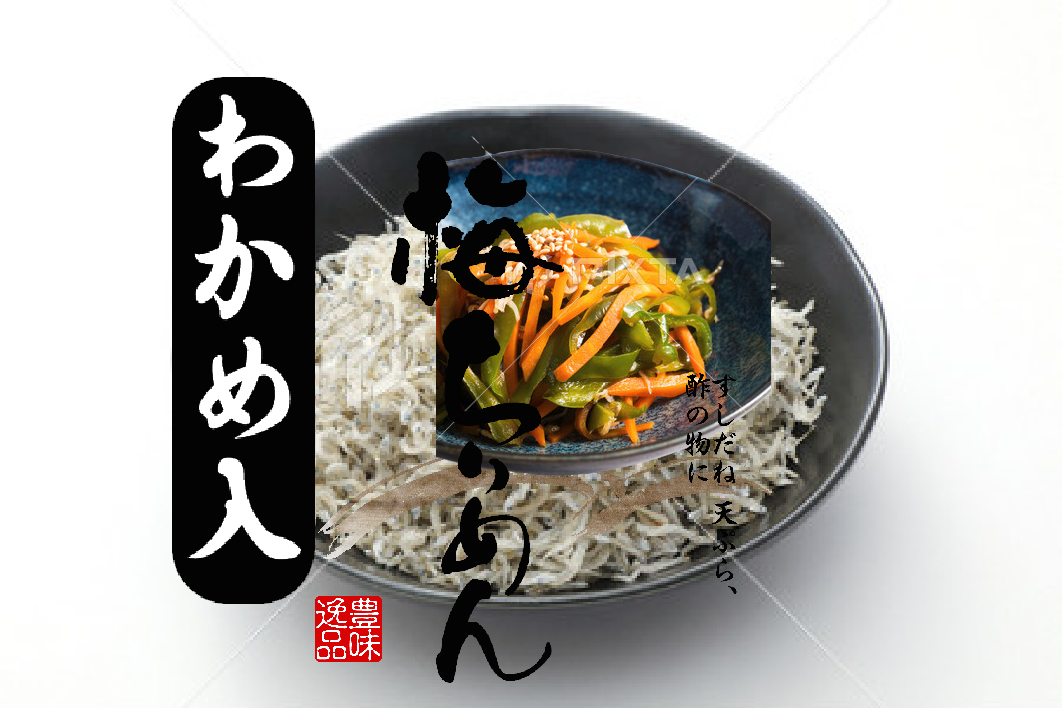
\includegraphics[scale=2]{src/pictures/zurag3.png}
	\caption{Жишээ-3}
\end{figure}

% Хавсралтын нэр. Хавсралт гэдэг үг агуулахгүй
\chapter{Кодын хэрэгжүүлэлт}
\section{Python}
\subsection{Гол script}
\lstinputlisting[language=Python, caption=Text-ээс PNG зураг үүсгэдэг script]{src/code/script.py}
\subsection{Business logic script}
\lstinputlisting[language=Python, caption=Combination үүсгэх бизнес логик код]{src/code/combination.py}
\lstinputlisting[language=JavaScript, caption=Фронтэнд хэсгийн компонент код]{src/code/front.vue}
\lstinputlisting[language=Python, caption=Датабазруу КРУД хийх]{src/code/crud.py}


%----------------------------------------------------------------------------------------
%   Хавсралтууд эндээс эхэлнэ
%----------------------------------------------------------------------------------------

\end{document}